\documentclass[border=10pt]{standalone}
\usepackage[svgnames]{xcolor}
\usepackage{amsmath}
\usepackage{pgfplots}
\pgfplotsset{compat=newest}
\usepackage[sfdefault]{FiraSans}
\usepackage{FiraMono}
\renewcommand*\familydefault{\sfdefault}
\begin{document}
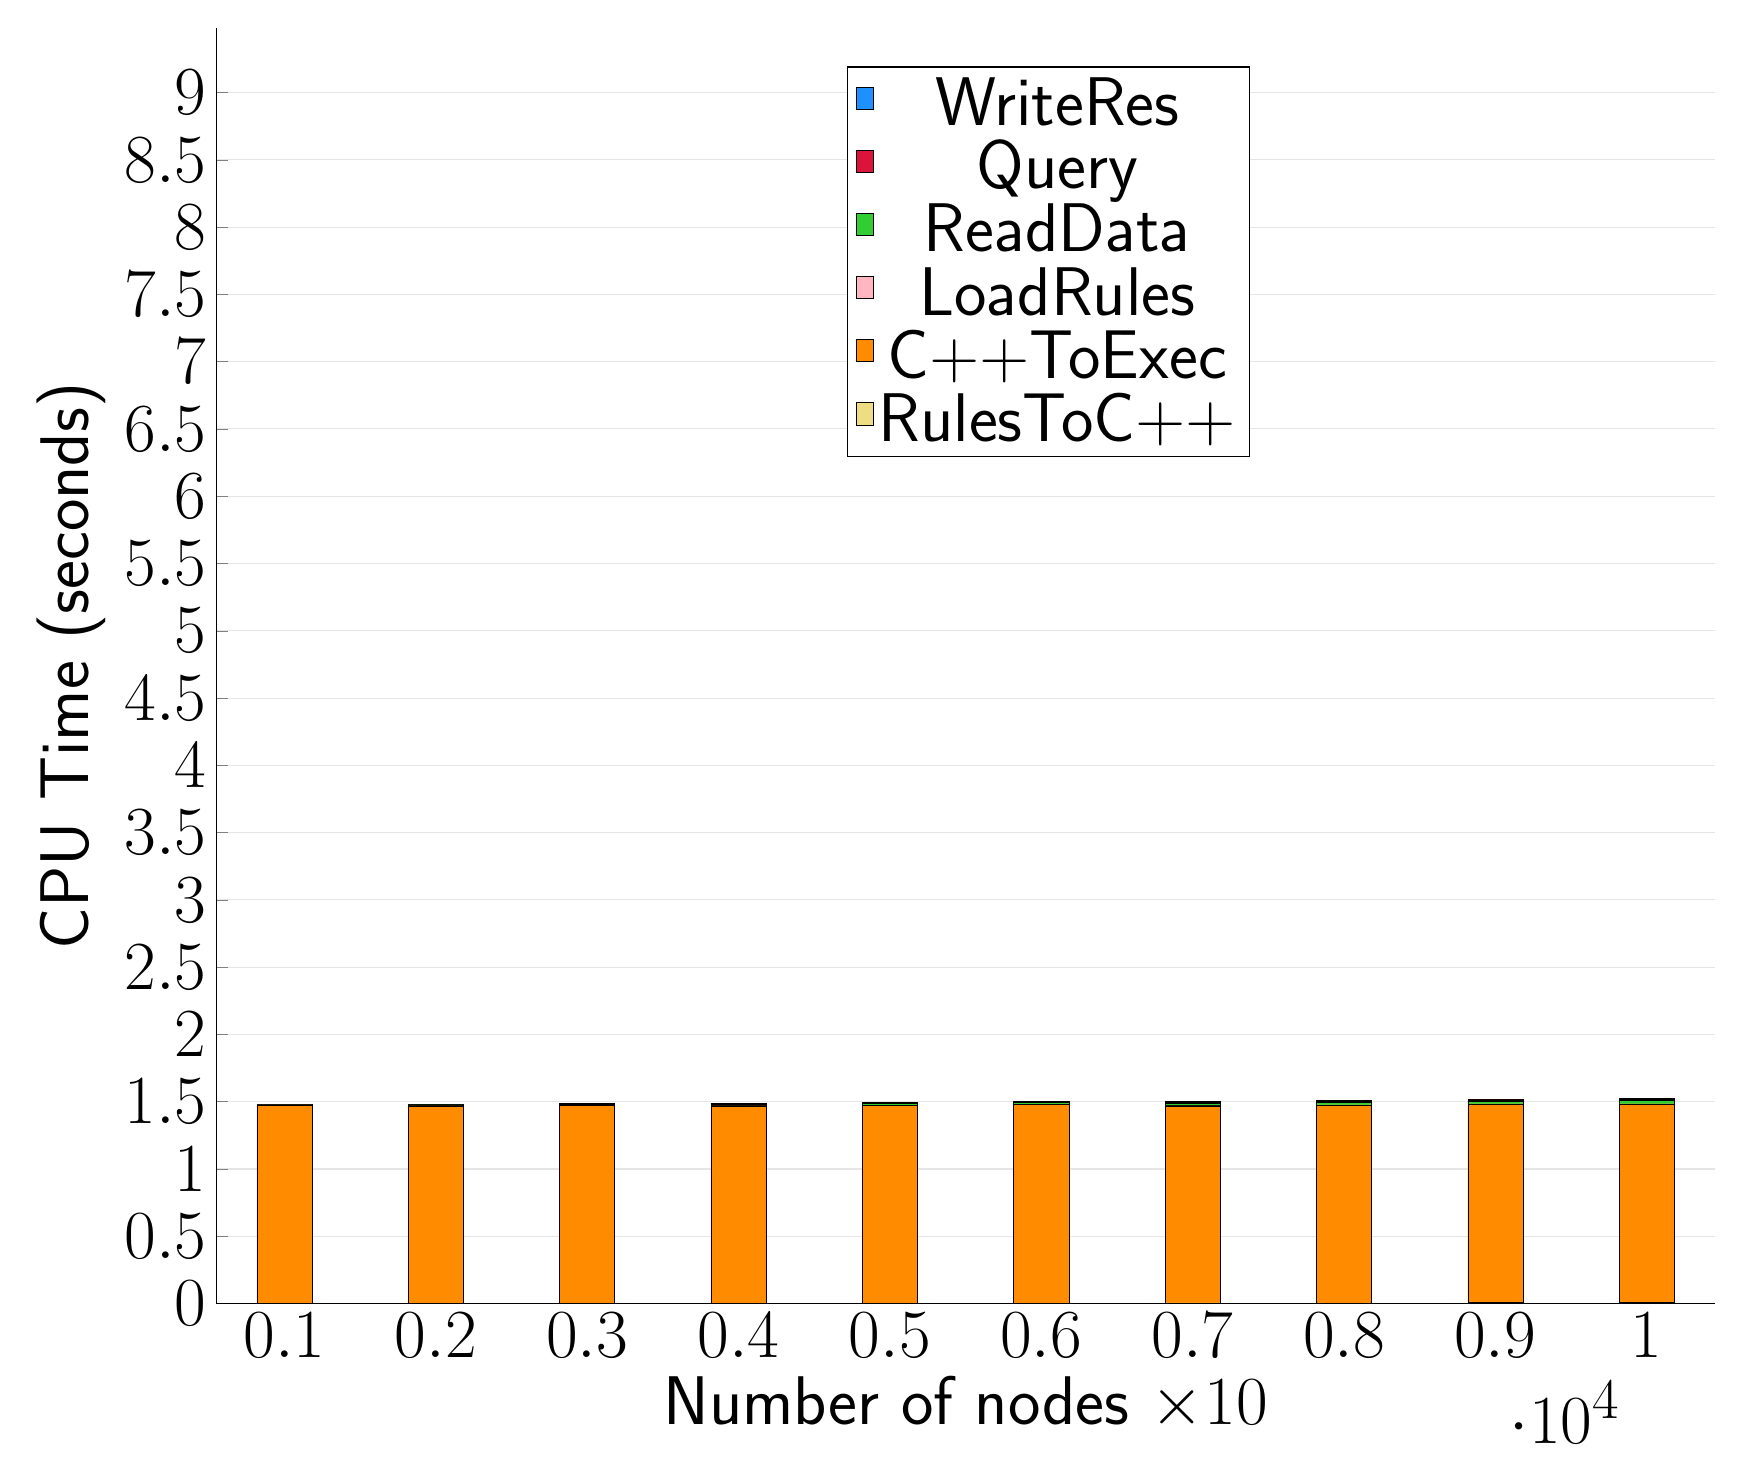
\begin{tikzpicture}
\begin{axis}[
   ybar stacked,
   width=1.7\textwidth,
   bar width=0.7cm,
   ymajorgrids, tick align=inside,
   major grid style={draw=gray!20},
   xtick=data,
   ymin=0, ymax=9.478,
   axis x line*=bottom,
   axis y line*=left,
   enlarge x limits=0.05,
   legend style={
       at={(0.69, 0.97)},
       anchor=north east,
       legend columns=1,
       font=\Huge,
   },
   ylabel={CPU Time (seconds)},
   xlabel={Number of nodes $\times 10$},
   label style={font=\Huge},
   tick label style={font=\Huge},
]
\addlegendimage{fill=DodgerBlue, draw=black, line width=0.2pt}
\addlegendentry{WriteRes}
\addlegendimage{fill=Crimson, draw=black, line width=0.2pt}
\addlegendentry{Query}
\addlegendimage{fill=LimeGreen, draw=black, line width=0.2pt}
\addlegendentry{ReadData}
\addlegendimage{fill=LightPink, draw=black, line width=0.2pt}
\addlegendentry{LoadRules}
\addlegendimage{fill=DarkOrange, draw=black, line width=0.2pt}
\addlegendentry{C++ToExec}
\addlegendimage{fill=LightGoldenrod, draw=black, line width=0.2pt}
\addlegendentry{RulesToC++}
\addplot +[fill=LightGoldenrod, draw=black, line width=0.2pt] coordinates {
(1000, 0.0020000000000000005)
(2000, 0.0020000000000000005)
(3000, 0.0020000000000000005)
(4000, 0.0)
(5000, 0.004000000000000001)
(6000, 0.0)
(7000, 0.006000000000000001)
(8000, 0.004000000000000001)
(9000, 0.008000000000000002)
(10000, 0.010000000000000002)
};
\addplot +[fill=DarkOrange, draw=black, line width=0.2pt] coordinates {
(1000, 1.4700000000000002)
(2000, 1.4679999999999997)
(3000, 1.47)
(4000, 1.47)
(5000, 1.47)
(6000, 1.4780000000000002)
(7000, 1.464)
(8000, 1.472)
(9000, 1.476)
(10000, 1.4740000000000002)
};
\addplot +[fill=LightPink, draw=black, line width=0.2pt] coordinates {
(1000, 0.000162)
(2000, 0.0001806)
(3000, 0.0001718)
(4000, 0.0001794)
(5000, 0.00016519999999999998)
(6000, 0.00017039999999999997)
(7000, 0.00017500000000000003)
(8000, 0.0001654)
(9000, 0.00016079999999999998)
(10000, 0.000172)
};
\addplot +[fill=LimeGreen, draw=black, line width=0.2pt] coordinates {
(1000, 0.0037700000000000003)
(2000, 0.0067308)
(3000, 0.009420000000000001)
(4000, 0.0126858)
(5000, 0.014588399999999998)
(6000, 0.0162232)
(7000, 0.0187934)
(8000, 0.0195762)
(9000, 0.021140399999999997)
(10000, 0.025245200000000002)
};
\addplot +[fill=Crimson, draw=black, line width=0.2pt] coordinates {
(1000, 0.001434)
(2000, 0.0025512)
(3000, 0.0040978)
(4000, 0.0049254)
(5000, 0.0061042)
(6000, 0.007317800000000001)
(7000, 0.008381)
(8000, 0.008890200000000001)
(9000, 0.0089306)
(10000, 0.010400200000000002)
};
\addplot +[fill=DodgerBlue, draw=black, line width=0.2pt] coordinates {
(1000, 0.0008460000000000001)
(2000, 0.0013428)
(3000, 0.0017036)
(4000, 0.0020724)
(5000, 0.0023284)
(6000, 0.0025958)
(7000, 0.0027987999999999997)
(8000, 0.0029826)
(9000, 0.0031342)
(10000, 0.0034005999999999993)
};
\end{axis}
\end{tikzpicture}

\end{document}
